\documentclass[
    iict, % Saisir le nom de l'institut rattaché
    il, % Saisir le nom de l'orientation
    %confidential, % Décommentez si le travail est confidentiel
]{heig-tb}

\usepackage[nooldvoltagedirection,european,americaninductors]{circuitikz}
\usepackage{hyperref} 

%\signature{mbernasconi.svg} TODO

\makenomenclature
\makenoidxglossaries
\makeindex

\addbibresource{bibliography.bib}

\usepackage{etoolbox}
\renewcommand\nomgroup[1]{%
  \item[\bfseries
  \ifstrequal{#1}{A}{Constantes physiques}{%
  \ifstrequal{#1}{B}{Groupes}{%
  \ifstrequal{#1}{C}{Autres Symboles}{}}}%
]}

\newcommand{\nomunit}[1]{%
\renewcommand{\nomentryend}{\hspace*{\fill}#1}}

\nomenclature[A, 02]{\(c\)}{\href{https://physics.nist.gov/cgi-bin/cuu/Value?c}
{Vitesse de la lumière dans le vide}
\nomunit{\SI{299792458}{\meter\per\second}}}

\nomenclature[A, 03]{\(h\)}{\href{https://physics.nist.gov/cgi-bin/cuu/Value?h}
{Constante de Planck}
\nomunit{\SI[group-digits=false]{6.62607015e-34}{\joule\per\hertz}}}

\nomenclature[A, 01]{\(G\)}{\href{https://physics.nist.gov/cgi-bin/cuu/Value?bg}
{Constante de gravitation universelle}
\nomunit{\SI[group-digits=false]{6.67430e-11}{\meter\cubed\per\kilogram\per\second\squared}}}

\nomenclature[B, 03]{\(\mathbb{R}\)}{Nombres réels}
\nomenclature[B, 02]{\(\mathbb{C}\)}{Nombres complexes}
\nomenclature[B, 01]{\(\mathbb{H}\)}{Quaternions}

\nomenclature[C]{\(V\)}{Volume constant}
\nomenclature[C]{\(\rho\)}{Indice de frottement sec}

\newacronym{gcd}{GCD}{Plus grand diviseur commun}
\newacronym{lcm}{LCM}{Plus petit multiple commun}
\newacronym{uon}{UON}{Unified Object Notation}
\newacronym{antlr}{ANTLR}{Unified Object Notation}
\newacronym{ebnf}{EBNF}{Extended Backus–Naur Form}

\newglossaryentry{heig-vd}{
    name=HEIG-VD,
    description={Haute École d'Ingénierie et de Gestion du canton de Vaud}
}
\newglossaryentry{hes-so}{
    name=HES-SO,
    description={Haute École Supérieure de Suisse Occidentale}
}
\newglossaryentry{latex}{
    name=latex,
    description={Un langage et un système de composition de documents}
}
\newglossaryentry{maths}{
    name=mathematics,
    description={Les mathematiques sont ce que les mathématiciens fonts}
}
\newglossaryentry{token}{
    name=token,
    description={C'est un segment de texte avec un type associé}
}
\newglossaryentry{grammaire}{
    name=grammaire,
    description={un fichier décrivant formellement un langage}
}
% Auteur du document (étudiant-e) en projet de Bachelor
\author{Vitor Vaz Afonso}

% Activer l'option pour l'accord du féminin dans le texte
\genre{male}

% Titre de votre travail de Bachelor
\title{Support du langage UON sous VS Code}

% Le sous titre est optionnel
\subtitle{Travail de Bachelor}

% Nom du professeur responsable
\teacher {Prof. Y. Chevallier (HEIG-VD)}

% Mettre à jour avec la date de rendu du travail
\date{\today}

% Numéro de TB
\thesis{7212}



\surroundwithmdframed{minted}

%% Début du document
\begin{document}
\selectlanguage{french}
\maketitle
\frontmatter
\clearemptydoublepage

%% Requis par les dispositions générales des travaux de Bachelor
\preamble
\let\cleardoublepage\clearpage
\authentification
\let\cleardoublepage\clearpage

%% Résumé / Version abbrégée
\begin{abstract}
    % Francais

% • le contexte,
En 2018, le professeur Yves Chevallier a imaginé un nouveau format de sérialisation proche de YAML et JSON nommé \Gls{uon}.
UON vise à rassembler toutes les caractéristiques utiles des formats de sérialisation les plus utilisés sur internet (XML, YAML et JSON),
en un seul format qui les englobe. Cela dans le but de le rendre adapté à la communication \Gls{m2m} pour des dispositifs embarqués de faibles puissances, jusqu'aux plateformes haut de gamme basées sur le cloud.

% • la problématique,
Ce Travail de Bachelor a pour objectif de permettre l'utilisation du langage UON dans l'éditeur de code VS Code, en créant une extension disponible depuis le Marketplace de Visual Studio Code.
Cette extension doit fournir à l'utilisateur, le support de langage permettant une meilleure rédaction d'un fichier UON.

Le support est fourni sur une implémentation de la grammaire issue de la spécification UON.
L'API de VS Code est directement contactée pour implémenter les fonctionnalités.
ANTLR est le générateur de parser qui a été choisi.
Le moteur de complétion antlr4-c3 est utilisé comme source principale des suggestions pour l'auto-complétion.

Au terme de ce projet, les points attendus du cahier des charges ont été effectués. Il s'agit de :
\begin{itemize}
    \item Disposer d'une grammaire du langage UON utilisable
    \item Implémenter une intégration continue
    \item Implémenter une coloration syntaxique
    \item Implémenter de l'auto-complétion
    \item Implémenter une outline view
    \item Implémenter l'affichage des informations au survol de la souris (Hover Information)
    \item Implémenter un Linter simple pour signaler des erreurs
\end{itemize}

% • perspectives et recommandations
Les perspectives concernant ce sujet sont vastes, mais des améliorations possibles à ce projet sont les suivants :
\begin{itemize}
    \item Implémenter les points du CDC dans la partie "si le temps le permet".
    \item Utiliser un langage server au lieu de l'API VS Code.
    \item Continuer à améliorer la grammaire et adapter les fonctionnalités en conséquence.
\end{itemize}
\end{abstract}

%% Sommaire et tables
\clearemptydoublepage
{
    \tableofcontents
    \let\cleardoublepage\clearpage
    \listoffigures
    \let\cleardoublepage\clearpage
    \listoftables
    \let\cleardoublepage\clearpage
    \listoflistings
}

\printnomenclature
\clearemptydoublepage
\pagenumbering{arabic}


%% Contenu
\mainmatter
\chapter{Introduction}
Ce projet de Bachelor consiste à fournir du support pour le nouveau langage de sérialisation UON, sous VsCode. Ce projet se veut expérimental. C’est-à-dire qu’aucun cadre précis sur sa réalisation n’a été établi et que les approches choisis sont libres tant qu’elles respectent le cahier des charges.
Dans les chapitres suivants, nous allons voir ce qui est fourni par VsCode pour élaborer et déployer une extension.
Les éléments à prendre en compte pour pouvoir fournir du support pour un langage.
Les aspects du langage UON à considérer dans le cadre de ce projet.
Et présenterons en détail l’implémentation d’une extension ainsi que ses fonctionnalités. Puis détaillerons les tests effectués.

\let\cleardoublepage\clearpage

\chapter{Cahier des charges}
Voici ci-dessous un résumé du cahier des charges :

\textbf{Extension}
\begin{itemize}
    \item Code source publié sur Github
    \item Fournir une intégration continue
    \item Déployer l'extension sur le marketplace
\end{itemize}

\textbf{Fonctionnalités à implémenter}
\begin{itemize}
    \item Syntax highligting
    \item Auto-complétion
    \item Document Outlining
    \item Hover Information
\end{itemize}

\textbf{Si le temps le permet}
\begin{itemize}
    \item Lint
    \item Formatter
    \item Converter
\end{itemize}

Ce projet se focalise uniquement sur l’éditeur de code VScode.
Il a donc été décidé de le réaliser en Typescript étant donné que VS Code extensions supporte 2 langages principaux (Javascript et Typescript).
Nous avons choisi les fonctionnalités attendues en choisissant celles paraissant utiles à avoir dans un premier temps et en prenant en considération la contrainte de temps.


\chapter{Pré-étude}

\section{L\textquotesingle implémentation de fonctionnalités}
VsCode fournit la possibilité d’ajouter du support pour un nouveau langage de programmation au travers d’implémentation de fonctionnalités. Ces fonctionnalités peuvent être classées en 2 catégories :

\section{Declarative language features}
Elles ajoutent un support d'édition de texte de base pour un langage de programmation.
Par exemple, les éléments suivants :

\begin{itemize}
    \item Syntax highlighting
    \item Snippet completion
    \item Bracket matching
    \item Bracket autoclosing
    \item Bracket autosurrounding
    \item Comment toggling
    \item Auto indentation
    \item Folding (by markers)
\end{itemize}

Il s’agit de fonctionnalités implémentées à l’aide de fichier de configuration.
Puis, elles doivent être enregistrées dans le fichier package.json du projet sous le champ \guillemotleft contributes\guillemotright \space \href{https://code.visualstudio.com/api/references/contribution-points}{ Contribution Point}.

\section{Programmatic language features}
Il s’agit de fonctionnalité plus riche donc plus complexe à implémenter (p.ex : \guillemotleft Hovers\guillemotright, \guillemotleft Go to Definition\guillemotright, \guillemotleft diagnostic errors\guillemotright, \guillemotleft IntelliSense\guillemotright \space et \guillemotleft CodeLens\guillemotright) et qui nécessite soit d’utiliser l’api vscode.languages.* qui expose des interfaces permettant de réaliser directement leur implémentation ou soit de les implémenter nous-mêmes au travers d’un langage serveur. 
Les avantages souvent mentionnés de la deuxième solution et que le langage server peut être écrit avec le langage que l’on souhaite et que cela permet aussi à d’autres éditeurs de texte compatibles avec le langage server d’utiliser ses fonctionnalités sans devoir les implémenter de nouveau. Mais comme points négatifs cette approche est plus complexe à implémenter et dans notre cas n’est pas un choix primordial.

\subsection{Langage server}
Pour être utiliser sur VSCode, un langage server à 2 partis :
\begin{itemize}
    \item \textbf{Un client} : C’est une extension écrite en Javascript ou Typescript qui à accès à tous les endpoints de VScode
    \item \textbf{Langage server} : Un outil d'analyse linguistique fonctionnant dans un processus séparé lancé
\end{itemize}

Le client et le serveur communiquent à l’aide du protocole LSP (pour \guillemotleft language server\guillemotright) dès que des informations riches devraient être fournies à l’éditeur.
Le langage server devrait donc ensuite pouvoir \guillemotleft consommer\guillemotright un parser pour traiter les fonctionnalités. C’est-à-dire être capable d’analyser un AST et de fournir une réponse adéquate.
L’implémentation d’un tel serveur peut être libre, mais des implémentations existent déjà. Telle que \guillemotleft LSP4\guillemotright implémenté en Java ou \guillemotleft Vscode-languageserver-node\guillemotright implémenté en Typescript qui n’est pas exclusivement réservé à VsCode comme son nom pourrait l’indiquer.
On remarque donc avec cette approche que 2 composantes existent (Le client et le serveur)
Un langage server peut être utilisé sur d’autre éditeur compatible. Mais le client devra être implémenté de nouveau.

\subsection{VsCode API (Direct implementation)}
L’autre approche et donc de communiquer directement avec l’api en s’inscrivant à des providers.
L’éditeur fera les requêtes aux providers lorsque nécessaire.

\begin{figure}[!ht]
    \begin{center}
        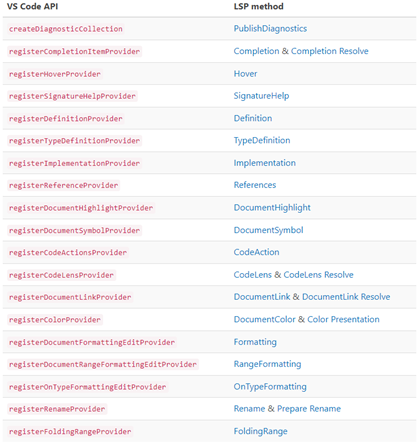
\includegraphics[width=10cm]{assets/figures/api-vscode.png}
    \end{center}
    \caption[API]{\label{test} blabla...}
\end{figure}

Ce schéma ci-dessus montre la correspondance des méthodes entre la première et seconde approche.
Beaucoup de possibilités et donc fourni, mais nous utiliserons uniquement les providers suivants :

\begin{itemize}
    \item \textbf{registerCompletionItemProvider}
          \subitem Pour afficher des suggestions de complétions
    \item \textbf{registerHoverProvider}
          \subitem Pour gérer le hover
    \item \textbf{registerDocumentSymbolProvider}
          \subitem Pour afficher les éléments dans la Outline View
\end{itemize}

\subsection{Parser}
Pour pouvoir analyser le code saisi par l’utilisateur, la création d’un parser est une approche souvent utilisée.
Cependant dans le cadre de son utilisation dans un éditeur/IDE, il devrait être \guillemotleft fault tolerant\guillemotright. C’est-à-dire que comme un parser normal, il doit générer un AST (abstract syntax tree), mais lors du parsing du code, il ne devrait pas s’arrêter dès la première erreur.
Car la plupart du temps, le code dans l'éditeur est incomplet et syntaxiquement incorrect, mais les développeurs s'attendent tout de même à ce que la complétion automatique et les autres fonctions de la langue fonctionnent.


\subsection{Grammaire}
Il faudra aussi élaborer une grammaire pour le langage de sérialisation UON utilisable par le parser.
Pour faciliter l’étape de l’analyse syntaxique (« Parsing »), cette grammaire pourrait être plus permissive, en particulier concernant les types attendus (Terminaux). Ainsi si l’utilisateur entre une valeur dont le type attendu est incorrect (par rapport aux spécifications du langage). Nous n’avons pas à traiter ce type d’erreur.

\section{Recherche d'extensions similaires}
Fournir du support pour un nouveau langage est une tâche relativement courante.
Il est donc relativement simple de trouver des extensions proposant un objectif similaire sur la marketplace.
Évidemment c’est donc une des premières choses qui ont été faites. Regarder les extensions similaires et particulièrement ceux touchant à des langages de sérialisation.

\subsection{Yaml}
UON étant un langage proche de YAML c’est vers son extension que je me suis dirigée en premier. Car il n’existe pas d’extension officielle, similaire pour le langage JSON.
Cependant j’ai vite compris que cela n’allait pas forcément être aussi évident. Car contrairement à JSON et YAML, UON intègre directement dans son langage des types définis. Ce qui fait que l’auto-complétion fournit par des JSON Schema dans l’extension YAML n’est pas vraiment applicable pour notre cas.
Aussi pour l’outline view. La création d’un symbol tree se fait à l’aide de fonction utilitaire très « privée » et complexe à reprendre est à adapté. En cherchant, j’ai vu que JSON utilise ces mêmes fonctions.
Cette direction a donc été écarté.

\section{Choix technologiques}
Comme expliqué précédemment, la catégorie d’une fonctionnalité va influencer son implémentation sous VsCode. Mais certaines de ces fonctionnalités pourraient être implémentées selon l’une ou l’autre approche en fonction de la complexité souhaitée, par exemple le  \guillemotleft code folding\guillemotright ou \guillemotleft autocompletion\guillemotright. Il est donc possible que lors du déroulement du projet que la solution jugée la plus intéressante soit privilégiée.

\subsection{Grammaire}
Une grammaire simplifiée de UON sera l’approche privilégiée au départ. Si nécessaire, elle pourrait être étendue.

\subsection{Parser}
Des outils permettant la génération d’un parser en fonction d’une grammaire existent et seront privilégiés. Si cette approche échoue alors soit l’implémentation d’un parser simple sera effectuée ou il faudra envisager une piste alternative.

\subsection{API}
L’implémentation d’un langage serveur n’étant pas une priorité et pour se concentrer sur la réalisation des fonctionnalités, l’approche de contacter directement l’api de VsCode sera choisi. Si le temps le permet, toute la logique du code concernant les fonctionnalités pourrait être déplacée dans un langage server. 

\section{Vscode}
Presque tout est customisable. Ce rapport ne va pas entrer en détail sur tout ce qui est possible de faire. Si besoin, VsCode fourni une multitude d’explication bien détaillée et fournie en exemple.

\section{UON}
UON est essentiellement un langage de sérialisation qui est un superset de JSON et un superset partiel de YAML. Il fournit des fonctionnalités supplémentaires utiles pour augmenter l'interopérabilité entre différents types de dispositifs.

\subsection{Pourquoi ?}
Son rôle est d’être utilisé dans l’industrie 4.0. Plus particulièrement dans la communication m2m (machine to machine) ainsi que pour l’IoT (Internet of Things).
Beaucoup d’informations circulent entre ces composants et leurs ressources sont limitées.
C’est ici que ce langage est intéressant. Car il a pour objectif d’encapsuler et représenter l’information avec le plus petit payload possible.
Pour cela UON permet :
\begin{itemize}
    \item De représenter les données sous forme humaine et binaire.
    \item Décrire le payload à travers d’un schéma de validation.
\end{itemize}
Son rôle est donc de représenter des données sous forme la plus minimale pour permettre l'interopérabilité entre machines.

\subsection{Design}
UON est complètement conforme avec JSON et partiellement avec YAML.

\subsection{Types}
Chaque élément est composé d’un type. Et chacun de ces types peut avoir des propriétés.
3 types de propriétés existent :
\begin{itemize}
    \item Presenentation properties.
    \item Validation propeties
    \item Application properties
\end{itemize}

\subsection{Schéma de Validation}
Une des propriétés uniques de UON est l’usage de schéma directement intégré dans le langage.
Le rôle de ce schéma et que les machines se mettent d’accord entre elles sur le format des données à respecter, diminuant ainsi le payload total et s’assurant de la validité des données.

\subsection{Liens}
La spécification comète du projet se trouve ici : \href{https://github.com/uon-language/specification/}{https://github.com/uon-language/specification/}
Et le dépôt du projet : \href{https://github.com/uon-language/specification}{https://github.com/uon-language/specification}


\chapter{Scope de la grammaire}
Pour pouvoir proposer du support pour un nouveau langage, il est nécessaire de savoir sur quoi celui-ci portera. Il est donc important préciser sur quels éléments du langage (grammaire) nous nous focaliserons.
Nous allons donc partir d’une grammaire la plus minimale possible tout en faisant attention à son extensibilité par la suite.
Cette grammaire se trouve dans le fichier UON.g4.

Elle est une adaptation de la grammaire écrite en Lark par l’ancien élève Stéphane Selim pour son travail de bachelor « Parser for a serialization language UON ». Son travail se trouve sur : 
\href{https://github.com/uon-language/uon-parser}{https://github.com/uon-language/uon-parser}

Elle sera complétée et améliorée après la mise en place des fonctionnalités attendus et si le temps le permet.

Les fonctionnalités implémentées s’appuieront sur cette grammaire. Ceci dans le but de rester cohérents entre eux.

\textbf{Rappel}
La grammaire actuelle nous permet de définir des maps, séquences dans le format json et yaml. D’ajouter des propriétés à des types et également la possibilité de définir un schéma.

\section{Modification}
\textbf{[TODO]}


\chapter{Implémentation}
Dans ce chapitre, nous allons explorer les aspects techniques concernant l’implémentation de fonctionnalités. Nous allons voir également les outils utilisés ainsi que le déploiement de l’extension sur le marketplace.
Ce travail reflète uniquement mon approche personnelle sur la matière. Et ne devrait pas être considérée comme l’unique manière de procéder. 

\section{Code}
Le code de l’implémentation est disponible sur le dépôt public suivant : \textbf{[pour l’instant privé]}
Est hébergé sous l’organisation : \textbf{[TODO]}
\textbf{Remarque} : L’implémentation détaillée dans ce rapport pourrait ne plus représenter l’état du dépôt, car ce projet est sujet à évoluer.

\section{Extension}
\dots

\section{Parser}
Une approche souvent prévilégié pour l’implémentation de fonctionnalités de langage est la génération d’un AST pour en tirer des informations et les utiliser. Pour le générer, un parseur est nécessaire. Étant donné que ce n’est pas le sujet de notre TB, je vais m’aider d’outil existant pour extraire le plus possible de complexité concernant ce sujet.

\subsection{ANTLR}
L’utilisation de ANTLR (ANother Tool for Language Recognition) comme générateur de parser a été choisie pour les raisons suivantes :
\begin{itemize}
    \item C’est un outil populaire est encore utilisé.
    \item Il est disponible en Typescript (\href{https://github.com/tunnelvisionlabs/antlr4ts}{antlr4ts}).
    \item Un moteur de complétion existe avec les parser générés avec antlr. Nous simplifions de grandes étapes pour implémenter l’auto-complétion (\href{https://github.com/mike-lischke/antlr4-c3}{antlr4-c3})
    \item Quelques exemples existent d’implémentation.
    \item La génération est simple. Pour générer un parser (et d’autres fichiers utiles), il suffit d’écrire un fichier contenant une grammaire valide.
\end{itemize}

\subsubsection{Grammaire}
Le fichier de grammaire doit respecter les points suivants : \textbf{[TODO]}

\textbf{Attention} : Utiliser des majuscules pour une règle, correspond à définir un \guillemotleft Lexer rule\guillemotright et utiliser des minuscules à un \guillemotleft Parser rule\guillemotright.

Quand le fichier de grammaire est écrit, il suffit de lancer le code suivant :

\begin{lstlisting}
    antlr4ts UON.g4 -no-listener -no-visitor -o generated -Xexact-output-dir
\end{lstlisting}

Il nous génère les fichiers suivants :
\begin{itemize}
    \item UON.interp
    \item UON.tokens
    \item UONLexer.interp
    \item UONLexer.tokens
    \item UONLexer.ts
    \item UONParser.ts
\end{itemize}

\subsection{Arbre (CST)}
\begin{figure}[!ht]
    \begin{center}
        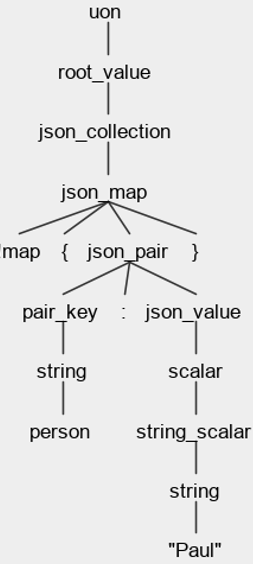
\includegraphics[width=10cm]{assets/figures/tree.png}
    \end{center}
    \caption[uon-tree]{\label{test2} blabla...}
\end{figure}


\chapter{Conclusion}

%%if
Bien que non nécessaire dans un rapport de Bachelor, la discussion finale d'un projet résume les résultats obtenus et dresse une conclusion objective du projet. Un manager de société est souvent amené à lire de nombreux rapport, il ne s'intéresse généralement qu'à l'introduction au contexte de l'étude et à sa conclusion.

Il est de coutume de signer la conclusion...
%%fi

\vfil
\hspace{8cm}\makeatletter\@author\makeatother\par
\hspace{8cm}\begin{minipage}{5cm}
    %%if
    % Place pour signature numérique
    \printsignature
    %%fi
\end{minipage}
\clearpage

\appendix
\appendixpage
\addappheadtotoc

%%if
\chapter{Première annexe}

Les annexes n'ont pas un contenu \underline{normatif} mais \underline{descriptif}. Tout contenu annexé ne doit pas être nécessaire à la bonne compréhension du travail.

Les annexes contiennent généralement :

\begin{itemize}
    \item les dessins mécaniques (mises en plan);
    \item les schémas électriques détaillés;
    \item des photographies du projet;
    \item des scripts et des extraits de code source;
    \item des documents techniques \pex \emph{datasheet};
    \item des développements mathématiques.
\end{itemize}
\section{Sous section}
\lipsum[1]
%%fi

\let\cleardoublepage\clearpage
\backmatter

\label{glossaire}
\printnoidxglossary
\printbibliography
\label{index}
\printindex

%%if
\clearpage
\Large\textbf{Colophon :}\par\normalsize
\thispagestyle{empty}
La qualité de cet ouvrage repose que le moteur \LaTeX. La mise en page et le format sont inspirés d'ouvrages scientifiques tels que le modèle de thèse de l'EPFL et celui des publications O'Reilly.

Les diagrammes et les illustrations sont édités depuis l'outil en ligne draw.io. Certaines illustrations ont été reprises dans Adobe Illustrator. Les représentations 3D sont exportées de SolidWorks et certains graphiques sont générés à la volée depuis un code source Python.

L'auteur fictive de ce document \emph{Maria Bernasconi} est un nom emprunté, par amusement, aux spécimens publiés par Postfinance.

Ce document a été compilé avec XeLaTeX.

La famille de police de caractères utilisée est \emph{Computed Modern} créée par Donald Knuth avec son logiciel METAFONT.
\vfil
Le Colophon est le dernier élément d'un document qui contient des notes de l'auteur concernant la mise en page et l'édition du document : il est parfaitement optionnel.
%%fi

\end{document}
